\section{Production Simulation}
\label{sec:productionSim}
 \begin{quotation}
"Production is a process of combining various material inputs and immaterial inputs (plans, know-how) in order to make an output for consumption. It is the act of creating an output, a good or service which has value and contributes to the utility of individuals."\cite{noauthor_production_2019}
 \end{quotation}
The definition above provides us with the basis of the production process. In it we can already start to differentiate separate sectors, such as the Procurement Department for getting the material inputs and the HR department for providing the know-how, the human factor in production. 

In this simulation we are going to focus on three very important indicators, namely \textit{totalProductQuality}, \textit{productCost} and \textit{productionProcessProductivity}. In order to derive these indicators we will need to analyze the factors that influence them and give them proper values. 

Firstly, \textit{totalProductQuality} (\gls{tPQ}) is considered a very important element in the production simulation, nevertheless it is a very volatile concept and thus challenging to define and implement in this simulation. Often defined as conformance to requirements \cite{crosby_quality_1979}, quality is an elusive factor of production, which we have tried to frame in order to serve the scope of this project.

% Start list with tProcureQ, as the othe factors are multiplicators of this factor
 Several factors that affect the \textit{totalProductQuality} in our CapitalismX simulation are listed below:
\begin{itemize}
\item productionTechnology (\gls{pT})
\item totalEngineerProductivity (\gls{tEP}) 
\item totalProcurementQuality (tProcureQ)
\item R\&D
\end{itemize}
The \textit{totalProductQuality} is influenced by many elements, that in principle belong to the extend of other departments in the company. To illustrate, \textit{totalEngineerProductivity} is included in the HR simulation, the \textit{totalProcurementQuality} is included in the procurement simulation, etc. 

These elements all correlate in order to give an estimation of the \textit{totalProductQuality} per product. In order to estimate this correlation we compiled the following formulas.
 \begin{equation}
\gls{pTF}=0.7+0.1 \cdot pT
 \label{eq:pT}
 \end{equation}
 
By using formula \ref{eq:pT} the impact that \textit{productionTechnology} has on the \textit{totalProductQuality} can vary from $0.8$ to $1.2$, we measure this in the \textit{productionTechnologyFactor} (pTF). Meaning that if the \textit{pT} is lower than level $3$ which is the normal, good conditions state, this newly calculated \textit{pT} will have a decreasing effect on the \textit{totalProductQuality}, and if it is higher than $3$ the effect will be positive.
\begin{equation}
\gls{RDF}= 0.95 + 0.05 \cdot R\&D
\label{eq:R\&D}
\end{equation}

A similar scaling has also been carried out for R\&D, in which the level of impact is between $1$ and $1.2$. Meaning that even if the player has the lowest level of \textit{productionInvestments}, he or she does not lower the \textit{totalProductQuality} as the level of R\&D does not impact it. Our company will have no \textit{productionInvestment} in the beginnings and that should not lower the \textit{totalProductQuality}. If R\&D is in the highest levels than it will maximally influence the \textit{totalProductQuality} by $1.2$ times.

\begin{equation}
\gls{pAF}= 0.95 + 0.05 \cdot pA
\label{eq:R\&D}
\end{equation}
The \textit{processAutomationFactor} is also calculated in the same way. This is because even if there are no investments in \textit{pA}, this does not mean that the process is bad, and this factor should affect the \textit{totalProductQuality} negatively. It only means that there are no futuristic automatization processes running. If \textit{processAutomation} is in high levels, it can improve our products quality with a factor of $1.2$. 

\begin{center}
\begin{equation}
tEQoW=\sum_{e \in EN}{QoW}
\label{eq:tEQoW}
\end{equation}
where \\
\gls{EN} = Set of hired engineers
\end{center}
Formula \ref{eq:tEQoW} allows us to measure the \textit{totalEngineerQualityofWork} by deriving the sum of the \textit{qualityOfWork}, for all engineers. The calculations for \textit{qualityOfWork} can be found in the HR simulation, formula \ref{QoW}.
\begin{equation}
tEP=tEQoW \cdot pAF
\label{eq:tEP}
\end{equation}
Equation \ref{eq:tEP} mentioned above, shows the calculation of the \textit{totalEngineerProductivity}. This variable is given the value of the product of \textit{totalEngineerQualityofWork} and \textit{processAutomation}. It is done so, because \textit{processAutomation} is developing the futuristic  aspect of production and the higher the \textit{processAutomation} is the higher the \textit{totalEngineerProductivity}. 

In order to converge all the above mentioned elements and to measure the \textit{totalProductQuality} per product, we have compiled the following equation. 

% Vertical lines are not needed, root can't be less than 0
\begin{equation}
tPQ_{perProduct} = tProcureQ \cdot pTF \cdot |\sqrt[10]{tEP}| \cdot  R\&DF
\label{eq:PQ}
\end{equation}
 We measure the \textit{totalProductQuality} as a product of the three factors that were defined above, and the most important factor \textit{totalProcurementQuality}. We have defined it as most important, because the base material and components of our product constitute a large part in determining its quality.
 The factor \textit{totalEngineeringProductivity}
 % The growth of the factor \textit{totalEngineeringProductivity} has been slowed down by putting it in the 10th root
 has been normalized by putting it in the square root of power $10$. 
 % I don't understand this sentence, I think it could be clearer
 To further support this normalization into the range of the other factors the absolute value of this operation has been calculated.
 
 Furthermore we will introduce the \textit{nrProducedProducts} (\gls{nPP}) variable. This variable is measured in terms of daily amount of units produced for every product. This variable is used when calculating demand in chapter \ref{}. %Janine where is this var used?
 An additional element of a product that we would like to explain is the \textit{launchDate}. By using the \textit{launchDate}, we can prioritize the production process, in the case of a capacity limit. Meaning, if we have two different smartphones in line to be produced, and the machines do not have enough capacity to produce them both, the smartphone with an earlier \textit{launchDate} would be produced first.

After giving you an understanding of our concept of  \textit{totalProductQuality}, in the following sections we will explain the elements that  are included in this formula, and also further concepts that apply to the production process.

\subsection{Production Technology Level}
We will focus on \textit{productionTechnology} in this chapter, as you will encounter all the other elements in the following simulations. \\
% Sure it's a Likert scale?
Table \ref{table:my-label}, explains the $5$ points Likert-Scale for measuring \textit{productionTechnology}. This scale has a range of $[1-5]$, where $1$ is the lowest value and $5$ the highest.

\begin{table}[ht]
\centering
\begin{tabular}{|c|l|}
\hline
 Range & \textit{productionTechnology}\\
\hline
 1 & Depreciated  \\
 2 & Old \\
 3 & Good conditions \\
 4 & Purchased more than 5 years ago  \\
 5 & Brand New\\
\hline
\end{tabular}
\caption{\textit{productionTechnology}}
\label{table:my-label}
\end{table}

The technology of the machinery used in production starts at level $5$, when all machinery is new. This level can change during the game, by either increasing or decreasing. The \textit{productionTechnology} level can decrease one level$(-1)$ over a $5$ years time-span, due to the effects of \textit{machineryDepreciation}. This index can decrease two levels$(-2)$, if a natural disaster such as a fire, flood or a hurricane occurs.\\
There are also possibilities to improve the \textit{productionTechnology} level after a certain period of time has passed. These actions are created to  positively influence the technology level of machinery.
\begin{itemize}
    \item Purchasing new machinery (level $5$) \\
Purchasing new machinery immediately sets the machine's technology level to $5$, the maximum level, because the machinery is new and it complies with the measures of eco-laws and safety regulations.
\item Maintaining \& repairing $(+1)$ \\
Maintaining a machine is a regular process in all production companies. In CapitalismX, maintenance is optional for each machine, and the player can select which machine to maintain for a certain price. The price for maintenance is fixed for every machine and it improves the \textit{productionTechnology} scale by one level. \\
Repairs are also very frequent processes in production companies. Machines do not always function properly, and after using them at full capacity for a period of time they need intervening actions in order to restore them into their optimal state. In this simulation, repairs also increase the \textit{productionTechnology} scale by one level, as repairing is necessary, but it does not offer additional features to the machine. Both these processes have a cost of $2,000cc$ per machine.

\item Upgrading ($+2$) \\
Upgrading a machine is a process that implements new, better features into the current machine.
The cost of upgrading a machine is $5,000cc$, because alongside with increasing the \textit{productionTechnology} scale by two levels, upgrading also allows increasing the individual \textit{machineCapacity} by $20\%$. 
\end{itemize}
When buying a new machine the prices will be set by the game mechanics. This price calculation will be decided on the capacity of each machine, since they will all have a \textit{productionTechnology} level equal to $5$. The \textit{purchasePrice} is calculated as the sum of the \textit{machinePrice} equal to $100,000cc$, with the \textit{machineCapacity (\gls{mC})} times $120\%$.  The supplementary $20\%$ of the price is added to the amount, as an additional payment for the retailer.
\begin{equation}
purchasePrice=(machinePrice+mC)\cdot 120\%
\label{eq:buyMachine}
\end{equation}
In this simulation it is also possible to sell your current machines. A player should choose this option if he is low on CapCoins, or has purchased too many machines and they are deteriorating. The selling price will be set by the game mechanics, accordingly with equation \ref{eq:sellMachine}.
\begin{equation}
resellPrice=(pT \cdot levelPrice_{PerPTLevel})+mC
\label{eq:sellMachine}
\end{equation}
\begin{center}
	where\\
	pT = \textit{productionTechnology} \\
	mC = \textit{machineCapacity}
\end{center}
In this formula, the selling price is calculated by multiplying the current \textit{productionTechnology} with a bench-marked value of $20,000cc$ per \textit{productionTechnology} level and adding the \textit{machineCapacity} value. It is formulated as such because when the player purchases a machine its cost varies in terms of capacity. Whilst, when selling a machine not only the capacity changes between machines but also the \textit{productionTechnology} level. And it is precisely our \textit{productionTechnology} level that accounts for the loss of value effect of the machinery, otherwise known as depreciation. 
\begin{equation}
machineryDepreciation= machinePrice - (pT \cdot levelPrice_{PerPTLevel})
    \label{eq:machineDepreciation}
\end{equation}

This approach of calculating depreciation effects is not linear, because we have to keep in mind that our machinery can be maintained or upgraded, which means they will improve their \textit{productionTechnology} level and depreciate later than other machines, which have not undergone these procedures.

\subsection{Production Investments}
The player can decide how to improve \textit{productionProcessProductivity} based on several \textit{productionInvestment} options. These investments are correlated with the measurements of several performance indicators in the production simulation. The player must use his instinct and business acumen to understand what metrics influence these investments and how. It is the player's decision to insert the amount of CapCoins, that he wants to invest. \\
The available \textit{productionInvestment} possibilities are:
\begin{itemize}
\item Research and Development (R\&D)
\item systemSecurity (\gls{sS})
\item processAutomation (pA)
\end{itemize}
These investments options are also measured in our standard $5$ points Likert-Scale. The difference in these options lies in the fact that they start at level $1$, considering that in the beginnings the company has no \textit{productionInvestments} operating. The increase or decrease of these indexes is dependent on the amount of CapCoins that is invested in them.
\begin{table}[ht]
\centering
\begin{tabular}{c|c|c}
\hline
 Level & Description & CapCoins$_{(cc)}$\\
\hline \hline

 1 & No Investment & $0cc$ \\
 2 & Bad & $ 5,000cc$\\
 3 & Normal & $10,000cc$ \\
 4 & Good & $15,000cc$ \\
 5 & Very good & $20,000cc$\\
\hline
\end{tabular}
\caption{Levels of Production Investments}
\label{table:prod-investments}
\end{table}
As illustrated in table \ref{table:prod-investments}, all three of these indices will be able to change their current level by investing the corresponding amount of money.\\
Despite these investments being made once, there will come to a point in time, when they will begin loosing their added value to the production process. This loss is represented by Figure \ref{fig:InvestmentGraph}, and its corresponding function is $f(x)=5\cdot\exp^{-x}$. We take in consideration the $x$ range from $0$ to $10$. This graph encompasses the phenomena of "loss of added value" that we wanted to convey.

\begin{figure}[ht]
\centering
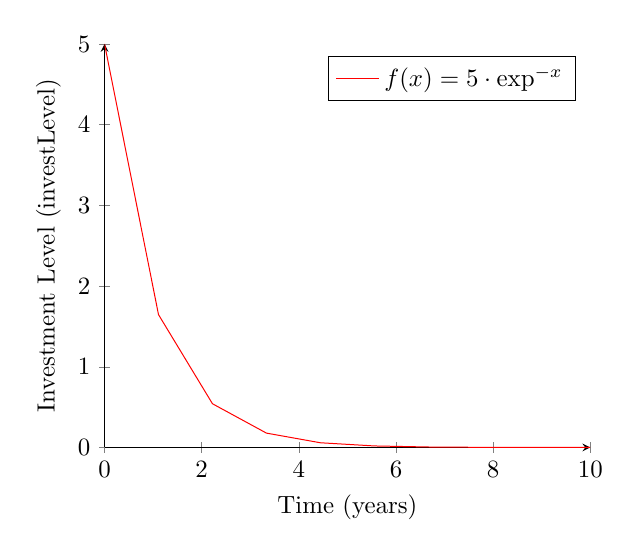
\begin{tikzpicture}[scale=0.9]
\begin{axis}[
    axis lines = left,
    xlabel = Time (years),
    ylabel = Investment Level (investLevel),
    grid style = dashed,
    legend pos=north east
]

\addplot [
    domain=0:10, 
    samples=10, 
    color=red,
]
{5*e^(-x)};
\addlegendentry{$f(x)=5 \cdot \exp^{-x} $}
\end{axis}
\end{tikzpicture}
\captionof{figure}{Production Investment Graph}	\label{fig:InvestmentGraph}
\end{figure}


In order to avoid the \textit{productionInvestment} to significantly lower the \textit{totalProductQuality}, the player must keep in mind to invest in these elements constantly over the duration of the game. Preferably, the \textit{productionInvestments} should be less than $5$ years apart, since the effect of an investment reaches $0$ after this time-span.

There is a special event, we have implemented regarding \textit{systemSecurity}.
If the \textit{systemSecurity} indicator falls below the $3^{rd}$ level threshold, incidents in the workplace and stealing inside the company will start to occur and they will negatively influence \textit{companyImage}. 

\textit{processAutomation} is another \textit{productionInvestment} option and it represents the company's direction towards more automated, futuristic processes. Its range is the same as the other \textit{productionInvestment} and is set by the amount of money invested. Nevertheless, it is a bit more complex as it needs to have some prerequisites fulfilled regarding \textit{employeeSkills}. In order to increase \textit{pA} according to the money invested, the player must have trained the employees in the production area, which means that the new technologies that will be implemented in production, will meet with employees that are trained to handle them. The possible trainings can be seen in section \ref{sub:KPI}. It is required to have at least $1$ production engineer trained, for each level of \textit{pA}. For instance, in order to invest and have \textit{pA} set in level $4$, at least $4$ production employees need to be trained in the production area.

All the simulation explained in this section will not be visible to the player, in order to increase the level of difficulty of the game and make the player more perceptive to the effect of these elements. 


\subsection{Production Costs}
\label{prodCosts_simulation}

To determine the \textit{totalProductCost} (\gls{tPC}), several components have to be taken into account, as demonstrated in Figure \ref{fig:productionCosts}. The first is \gls{tCC}
which is the total of all component's costs, since we need several components in order to have one end product. The overall employee salary would be included in the equation, since all employees, no matter in which department they work in, give an input and add value to the product. But we have decided to separate costs according to departments, that is why the employee salaries will be included in the HR costs. Another cost that we have included in our simulation are the \textit{Eco-Costs}. You can find the details regarding the \textit{Eco-Costs} calculation in section \ref{sec:compEco-idex}. Furthermore we incorporated \textit{purchasedAssetsCosts}. 
\begin{equation}
       VC = \sum_{n=1}^{n=5}tCC_{perProduct} + ecoCosts_{perProduct}
   \end{equation}

Since machinery is purchased we have to account this expense to \textit{purchasedAssetsCosts}, which is part of the \textit{Fixed Costs}. \textit{Fixed Costs (FC)} like \textit{machineryDepreciation} costs or rent are also included because they are inevitable expenses that are present in every production company. 
% this is not entirely clear because we didn't introduce facilitiyRent and purchasedAssetCosts
% I think we should rather use the machinery fixed cost here
\begin{equation}
   \begin{aligned}
 FC = facilityRent + purchasedAssetCosts \\ +machineryDepreciationCosts
   \end{aligned}
   \end{equation}

\begin{figure}[H]
	\centering
		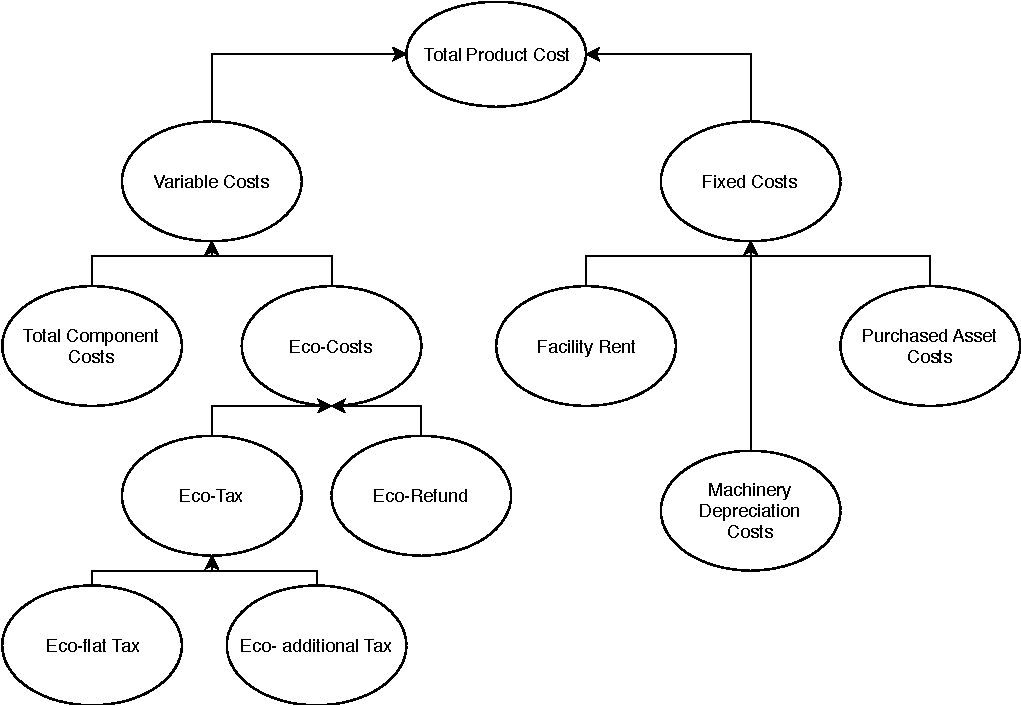
\includegraphics[scale=0.55]{images/ProductionCosts.pdf}
	\caption{Composition of \textit{totalProductCost}}
	\label{fig:productionCosts}
\end{figure}
All the above mentioned costs, add up to two major categories, \textit{variableCosts} and \textit{fixedCosts}. Together they compose the \textit{totalProductCost}. As demonstrated in equation \ref{eq: PC/u} the fixed costs are divided by the number of units that the player is going to produce, since the index that we are defining the \textit{totalProductCost} is calculated for each product in the set of products $P$.
% we introduced the set P for the products in the glossary so we can use it here (I added it)
\begin{equation}
	totalProductCost_{per Product}= VC + \frac{FC}{nr.Products} % nr. products = |P| 
	\label{eq: PC/u}
\end{equation}
By observing the above equation, we have described how the costs are simulated in the production process. 


\subsection{Pricing and Selling of Goods}
\label{sec:pricing_mechanics}
Part of the production simulation is the product view. Here the player can get an overview about the costs of every single component. Also, the user can define the market price for selling and the quantity to produce. This view is displayed in table format for convenient reading in table \ref{table:pricingView}.
\begin{table}[ht]
\centering
\begin{tabular}{|c|c|c|c|c|c|}
\hline
 Products & \begin{tabular}{@{}c@{}}Qty to \\ Produce\end{tabular} & \begin{tabular}{@{}c@{}}Amount \\ in Stock\end{tabular} & \begin{tabular}{@{}c@{}}Total Product \\ Costs\end{tabular} & \begin{tabular}{@{}c@{}}Sales Price \\ (per Product)\end{tabular} & \begin{tabular}{@{}c@{}}Profit \\ Margin\end{tabular} \\ \hline
 Product A &  & 12 & 332,56 &  & XX.X\% \\ \hline
 Product B &  & 554 & 62,05 &   & XX.X\% \\  \hline
 Product C &  & - & 164,67 &   & XX.X\% \\ \hline
\end{tabular}
\caption{Pricing View for the Player}
\label{table:pricingView}
\end{table}
The first column, "Product" displays the name of a product, that the player when he or she choose the product portfolio. The number of rows depends on the number of products the player added to the product portfolio.

The "Qty to Produce" field is an input field where the player can type in an integer value. The quantity depends on two different factors: the total \textit{machineCapacity} and the total \textit{warehouseCapacity}. If the amount entered by the player is larger than the accumulated sum of the \textit{machineCapacity}, then the player gets an error message: "Your machinery capacity is not sufficient. Either produce a smaller amount or buy new machinery". This is calculated as follows in function \ref{calc:machineryCapacity1} and \ref{calc:machineryCapacity2}.
\begin{equation}
\label{calc:machineryCapacity1}
   If~entered~amount \geq totalMachineCapacity, 
\end{equation}
whereas 
\begin{equation}
\label{calc:machineryCapacity2}
    Total~machineCapacity = \sum machineCapacity
\end{equation}

Also, the amount entered must not exceed the total \textit{warehouseCapacity}. The total \textit{warehouseCapacity} is determined as seen in chapter \ref{warehouse_simulation}. To calculate the maximum amount of products that can be produced, the number of stored products needs to be subtracted from the total \textit{warehouseCapacity}, as shown in function \ref{maxValueToProduce}:
\begin{equation}
\label{maxValueToProduce}
    Maximum~value~of~"Qty~to~Produce" = (nWH \cdot cWH) - nSP
\end{equation}

The next two fields are no input fields but serve the user in order to determine the quantity of products to produce and to define a market price to sell the product. First, the information field "Amount in Stock" displays the player the amount of each product in the warehouse(s), so $nSP_{per Product}$. The column "Total Product Costs" shows the player the total cost he or she expended for the producing the product and buying its components, which corresponds to the 
$totalProductCost_{perUnit}$. The calculation can be found in chapter \ref{prodCosts_simulation}, function \ref{eq:PQ}.

Moreover, the "Sales Price (per Product)", so the $productSale_{salesPrice}$ field is an input field where the player can type in a price in currency CapCoins for each product. The price is restricted to a float value with two decimals and a maximum of 99,999.99.
Last but not least, the field "Profit Margin" shows the profit margin for the respective product, which can be calculated as follows in function \ref{profitMargin}:
\begin{equation}
\label{profitMargin}
    Profit~Margin = \frac{salesPrice{pS} - tPC}{salesPrice{pS}} \cdot 100
\end{equation}
This value gives the player possible insights about his or her pricing strategy, as a high profit margin should only be used when using the components with the best \textit{baseQuality} and \textit{ecoIndex} and when also the own company's eco-index and \textit{customerSatisfaction} is very high.

As further clarified in chapter \ref{warehouse_simulation}, the products produced per day are first collected in the warehouse and sent out to the market in the next day. For the player, no further intervention is needed. Once determined how many products to produce, the selling process starts automatically.

\subsection{Performance metrics}
\label{sub:PM}

In this section we are going to present some important metrics that help us understand how, not only quality but also the \textit{productionProcessProductivity} is measured in our game. In order to measure production productivity we also need to define  \textit{manufactureEfficiency}. 

\textit{manufactureEfficiency} is measured by dividing the number of goods produced, on a monthly basis, by the current number of machines times their average capacity to produce in a month. This measure is important as it shows the player the rate in which the machinery is being utilized. This index has a range of $[0-1]$,which means if \textit{mE} is close to $1$ the usage of the machinery is optimal, but if this index is low, the player should realize he should either produce more or sell some of the machinery in order to keep efficiency high and not waste resources.
\begin{equation}
mE_{perMonth}= \frac{nr. units Produced_{perMonth}}{nr. Machines\cdot avg. Capacity_{perMonth}}  
\label{eq: ME}
\end{equation}

\textit{productionProcessProductivity} (\textit{pPP}) is an indicator of the efficiency of our production  process. It is based on \textit{productionTechnology} and \textit{totalEngineerProductivity} as indicators of the quality of the process and \textit{manufactureEfficiency} as an indicator of the efficiency of the manufacturing process.
\begin{equation}
pPP_{perMonth}= (pT + |\sqrt[10]{tEP}|) \cdot mE_{perMonth}
\label{eq:PPP}
\end{equation}
In this equation, we are going to handle the value of \textit{tEP} in the same manner as we handled it in \textit{tPQ}, by taking the absolute value of its square root to the power of 10. Sequentially, in order to normalize \textit{pPP} we calculate according to the following normalization function, where the \textit{max} and \textit{min} of our \textit{pPP} are $3.2$ and $0.2$ accordingly.

\begin{equation}
   pPP_{N\footnotemark}= \frac{x-min}{max-min}=\frac{pPP-0.2}{3.2-0.2}
\end{equation}
\footnotetext{N: index is normalized in the range of $[0-1]$}
 
To conclude, in our production simulation we explained several elements that influence the production process. These elements include machinery, possible investments and performance metrics. All of these elements derive to the two most important indicators, which are \textit{productQuality} and \textit{productionProcessProductivity}. By creating these indicators we have scratched the surface of manufacturing as a process, but they do provide a strong basis in order to provide a successful Production Simulation. 